\section{Tracking}
The tracking of objects with the KINECT System is done in five different steps. 
\begin{enumerate}
\item Take the Infrared (IR) image and the depth image with the KINECT System
\item Track the fiducials in the IR image
\item Convert the position of fiducials, which is given in pixels to mm
\item Identify the fiducials with respect to the reference model of the tracked object
\item Create the transformation matrix
\end{enumerate}
The KINECT System takes two different images. One infrared image and one image which represents the depth. While the values of the pixels in the infrared images are a decimal value between zero and one, the values of the depth images holds the actual depth in mm. In the end, we want to estimate the position of an object. This is done by placing fiducials on the object. This fiducials reflect the infrared light in a strong way, which appears in the infrared images as a bright dot. These dots can be tracked in the images and the position can be calculated. By knowing the distances between the fiducials on the object (stored in a reference model) and comparing these distances with the measured distances between the tracked points, we can determine the actual position of the object in the three dimensional space.
\\ \\But as in any real system, we have to deal with distortions. There are two big main problems:
\begin{enumerate}
\item Not only the fiducials can appear as bright dots. Also light from the sun or reflections of the infrared light from other objects can appear as bright dots in the image.
\item The distance measurement, which is used for creating the depth image, sometimes has problems to measure the right distance. In this cases, the distance for that point is zero. This is mostly the point, when a material reflect the infrared light in a strong way, which is nearly always true for the fiducials.
\end{enumerate}
To track only the fiducials and not some distortions, some filtering is done. To simplify the filtering, some parameters are set before the measurement starts:
\begin{itemize}
\item threshold for converting IR image from grayscale to black and white
\item minimal distance between object and camera in mm
\item maximal distance between object and camera in millimeters
\item minimal size of the fiducials in pixel
\item maximal size of the fiducials in pixel
\item scan area, in which the object will appear 
\end{itemize}
These settings can be set via a GUI, which also shows the scan area (in yellow) and the found fiducials. This is illustrated in \figref{fig:KINECT_GUI_screenshot}.
\begin{figure}[!t]
\centering
\includegraphics[width=3.5in]{KINECT_GUI_screenshot.PNG}
\caption{The GUI with the preview of the KINECT System and the parameters.}
\label{fig:KINECT_GUI_screenshot}
\end{figure}
With these parameters, the following filtering steps are performed:
\begin{enumerate}
\item Converting the IR image from gray scale to black and white. This is done by interpreting every pixel which is below the brightness the threshold as black and every pixel with a brightness over or equal the threshold as white.
\item Every white pixel which is to near to the camera or to wide from the camera is deleted (switched to black). For the actual distance, the depth image is taken. 
\item Every white pixel outside of the scan area is turned to black. 
\end{enumerate}

These three steps are shown in \figref{fig:KINECT_filtering1}, where step 1 is the original IR image, step 2 is the image converted to black and white, step 3 is the image, where the pixels which are to near or to wide away are deleted (note, that because of distortions in the depth image, the pixels in the lower left of the image are still there) and in step 4 all pixels outside of the can area are deleted.
In the next processing step, the pixels are clustered. The clustering groups all pixel, which are connected to each other to one group (see \figref{fig:KINECT_filtering2}). For each cluster, the following values are calculated:
\begin{itemize}
\item The area size of the pixels
\item The x and y coordinate (in pixels) of the middle of the pixel area
\item The bounding box for the pixel area. This describes the smallest possible rectangle,   
 which surrounds the pixel area, without crossing a pixel.
\end{itemize}
Now, for each cluster, the area size is checked, and if the area is in the specified region, the cluster is identified as a fiducial. As soon as the fiducial is identified, the x and y coordinates are stored in a vector. Because of the fact, that the depth image holds no information for the exact location of the fiducials, depth is calculated by the mean value of the depth of the pixels, which surrounds the fiducial. To simplify this process, the bounding box is used, to get the pixels from the depth image, which are outside of the fiducial, but close to it (see \figref{fig:KINECT_depthImg}).
\begin{figure}[!t]
\centering
\includegraphics[width=3.5in]{KINECT_filtering1.jpg}
\caption{The four steps of the filtering. 1: original IR image. 2: After converting to black and white. 3: Deleting all pixels which are to wide or to near from/to the camera. 4: Deleting all pixels outside of the scan area.}
\label{fig:KINECT_filtering1}
\end{figure}
In the last step, from measuring the position of the fiducials, the x and y component of the fiducials are converted from pixels to millimeters with the help of the intrinsic matrix. 
\begin{figure}[!t]
\centering
\subfloat[Pixels in clusters. Red: Boundingbox of each cluster]{\includegraphics[width=3.5in]{KINECT_filtering2.jpg}%
\label{fig:KINECT_filtering2}}
\hfil
\subfloat[Depth image with bounding boxes around the fiducials.]{\includegraphics[width=2.5in]{KINECT_depthImg.jpg}%
\label{fig:KINECT_depthImg}}
\caption{Identification of the bounding boxes of the fiducials.}
\label{fig:merged}
\end{figure}
Until this point, we have on the one side the reference model and on the other side normally four tracked fiducials, each with their x, y and z components. But we don’t know, which tracked fiducials corresponds to which fiducial in the reference model. To calculate the translation and rotation of the tracked object relative to the camera, we have to identify each tracked fiducial with respect to the fiducials in the reference model. 
This is done by calculating the distances between all points (this is done with the reference model and with the tracked fiducials). To avoid problems with measuring errors, distances in the tracked system, which are to similar are sorted out. To identify all fiducials, at least 4 distances have to remain. By comparing the distances between the tracked fiducials and the fiducials in the reference model, we can create connections between the points and identify the fiducials. This is shown in \figref{fig:KINECT_identify1} and  \figref{fig:KINECT_identify2} (but with only three fiducials and therefore three distances). For each distance from the reference system, the matching distance from the tracked system is searched. 
\begin{figure}[!t]
\centering
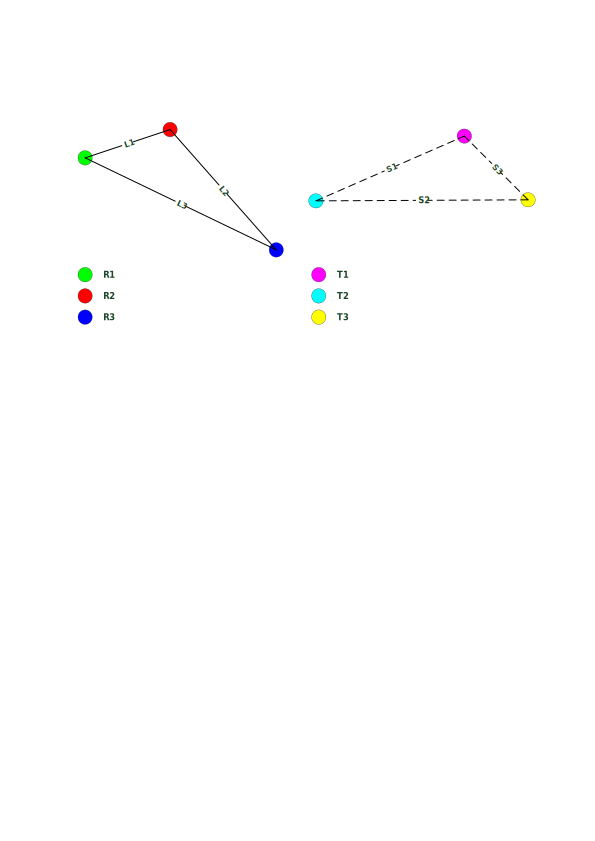
\includegraphics[width=3.5in]{KINECT_identify1.jpg}
\caption{Reference model (left) and tracked fiducials (right)}
\label{fig:KINECT_identify1}
\end{figure}
After that, a solution is searched which holds for each point of the reference system a point of the tracked system in a way, that the matching distances are made from the same points. The algorithm is pictured in  \figref{fig:KINECT_identify2}. The first point from the reference system (green) is taken and it is stored, which points from the tracked system it can be (cyan and yellow). Then the algorithm searches for the next distance, where the point one (green) appears. Then it checks if the yellow or the cyan point appears in the distance from the tracked system. The point which appears, corresponds to the first point. This is done for all three points from the reference system.
\begin{figure}[!b]
\centering
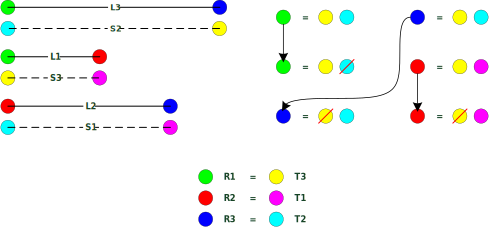
\includegraphics[width=3.5in]{KINECT_identify2.jpg}
\caption{Algorithm for identifying the points from the tracked system}
\label{fig:KINECT_identify2}
\end{figure}
The last process is to generate the transformation matrix out of the tracked points. To define a translation and rotation of the object, we first have to define a coordinate system for the object. The coordinate system is based on the points from the reference system, where the first point is used as base. The three unit vectors are created with the formulas below:
\begin{align}
\vec{e}_{x} &= \frac{\vec{p}_{2} - \vec{p}_{1}}{\left |~ \vec{p}_{2} - \vec{p}_{1} ~\right |} \\
\vec{s} &= \langle\vec{e}_{x},\vec{p}_{3}-\vec{p}_{1}\rangle\vec{e}_{x} \\
\vec{e}_{y} &= \frac{\vec{p}_{3} - \vec{p}_{1} - \vec{s}}{\left |~ \vec{p}_{3} - \vec{p}_{1} - \vec{s}~\right |} \\
\vec{e}_{z} &= \frac{\vec{e}_{x} \times \vec{e}_{y}}{\left |~\vec{e}_{x} \times \vec{e}_{y}~\right |}
\end{align}
This simple definition makes the calculation of the transformation matrix for the tracked points really easy. By defining the point $\vec{p}_{1}$ from the tracked system as base, the same formula can be used for the tracked points as it was used for the reference system. 